\documentclass[lettersize,journal]{IEEEtran} % package ieeetran, tlmgr install ieeetran avec TexLive
\usepackage{amsmath,amsfonts}
\usepackage{algorithmic}
\usepackage{algorithm} % package algorithms
\usepackage{array}
\usepackage[caption=false,font=normalsize,labelfont=sf,textfont=sf]{subfig} % package subfig
% On a aussi besoin du package caption
\usepackage{textcomp}
\usepackage{stfloats} % package sttools
\usepackage{url}
\usepackage{verbatim}
\usepackage{graphicx}
\usepackage{tikz}
\usepackage{cite}
% Aussi besoin de la font pcrr7t qui est dans le package courier
\hyphenation{op-tical net-works semi-conduc-tor IEEE-Xplore}
% updated with editorial comments 8/9/2021

\begin{document}

\title{Comparaison de différents routages pour les réseaux RTC}

\author{IEEE Publication Technology,~\IEEEmembership{\textsc{Fraty} Quentin, \textsc{Barniaudy} Maxime, \textsc{Maillet} Nathan,~IEEE,}
        % <-this % stops a space
\thanks{This paper was produced by the ENSEEIHT ASR Students.}% <-this % stops a space
\thanks{Manuscript received January 20, 2023; revised January 21, 2023.}}

% The paper headers
\markboth{N7's Journal of Network Architectures,~Vol.~1, No.~1, January~2023}%
{Shell \MakeLowercase{\textit{et al.}}: A Sample Article Using IEEEtran.cls for IEEE Journals}

\IEEEpubid{0000--0000/00\$00.00~\copyright~2023 IEEE}
% Remember, if you use this you must call \IEEEpubidadjcol in the second
% column for its text to clear the IEEEpubid mark.

\maketitle

\begin{abstract}
\end{abstract}

\begin{IEEEkeywords}
\end{IEEEkeywords}

\section{Introduction}
\IEEEPARstart{O}{ualid} 

\section{Réponses aux questions \& État de l'existant}
\subsection{Réseau sémaphore de la topologie considérée}

        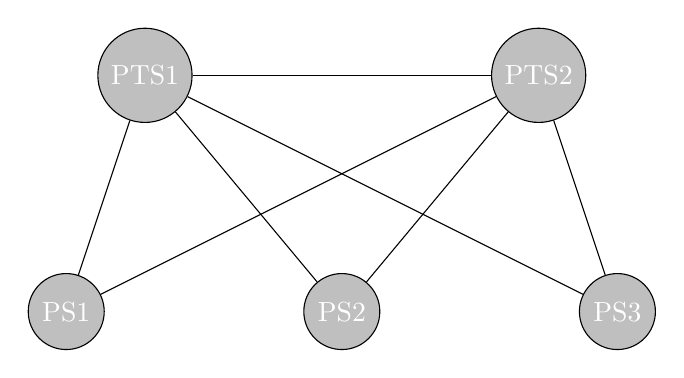
\begin{tikzpicture}
                \node[circle,draw,text=white,fill=lightgray] (PTS1) at (1,3){PTS1};
                \node[circle,draw,text=white,fill=lightgray] (PTS2) at (6,3){PTS2};
                \node[circle,draw,text=white,fill=lightgray] (PS1) at (0,0){PS1};
                \node[circle,draw,text=white,fill=lightgray] (PS2) at (3.5,0){PS2};
                \node[circle,draw,text=white,fill=lightgray] (PS3) at (7,0){PS3};

                \draw[-] (PTS1) -- (PTS2);
                \draw[-] (PTS1) -- (PS1);
                \draw[-] (PTS1) -- (PS2);
                \draw[-] (PTS1) -- (PS3);
                \draw[-] (PTS2) -- (PS1);
                \draw[-] (PTS2) -- (PS2);
                \draw[-] (PTS2) -- (PS3);
        \end{tikzpicture}

\subsection{Informations nécessaires à un routage par partage de charge}
% question de l'exam

\subsection{Informations nécessaires à un routage adaptatif}
% question de l'exam

\subsection{Routage des messages MTP-3}
% question de l'exam

\subsection{Transfert d'appels}
% question de l'exam

\section{Outils et modèles}
\section{Résultats}


\section{References Section}


\end{document}


